\documentclass[main.tex]{subfiles}
\begin{document}

\begin{frame}
\frametitle{Estimating the states}

The forward algorithm calculates $p(S)$ by marginalising the state vector $X$ out of the joint distribution $p(S,X)$.

\vspace{0.5cm}

But how do we estimate the state? One criterion is to choose the states, $X_1,X_2,...,X_T$ such that:

\vspace{0.5cm}

\begin{equation}
    X_1, X_2, ..., X_T = \argmax_{X_1, X_2, ..., X_T}{p(X_1,X_2,...,X_T,S_1, S_2,...,S_T)}
\end{equation}

\vspace{0.5cm}

But a brute force search is $O(N^T)$!

\end{frame}

\begin{frame}
\frametitle{The Viterbi algorithm}

Instead, we use a dynamic programming algorithm called the \textit{Viterbi} algorithm.

\vspace{0.5cm}

Starts at the beginning of the time series, and, in each subsequent time, it calculates:
%
\begin{equation}
    v_t(i) = \max_{X_1, X_2, ..., X_{t-1}} p(X_1, X_2, ..., X_{t-1}, X_t=i, S_1, S_2, ..., S_{t-1}, S_t).
\end{equation}
%
This can be calculated recursively as:
%
\begin{equation}
    v_t(i) = \left[\max_{j} v_{t-1}(j) p(X_t=i|X_{t-1}=j)\right] p(S_t|X_t=i).
\end{equation}
%
We also record which path led us here:
%
\begin{equation}
    \psi_t(i) = \argmax_{j} v_{t-1}(j) p(X_t=i|X_{t-1}=j).
\end{equation}
    
\end{frame}

\begin{frame}
\frametitle{Viterbi in action}

\begin{center}
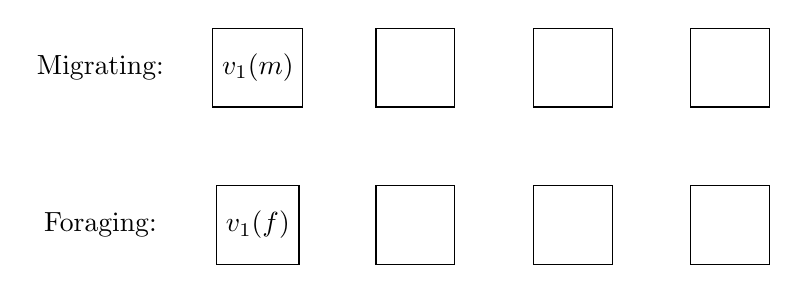
\begin{tikzpicture}[node distance=2cm, block/.style={draw, minimum width=1cm, minimum height=1cm}]

  % First row
  \node[block] (A1) {$v_1(m)$};
  \node[block, right of=A1] (A2) {};
  \node[block, right of=A2] (A3) {};
  \node[block, right of=A3] (A4) {};

  % Second row
  \node[block, below of=A1] (B1) {$v_1(f)$};
  \node[block, right of=B1] (B2) {};
  \node[block, right of=B2] (B3) {};
  \node[block, right of=B3] (B4) {};

  % Labels
  \node[coordinate, left of=A1] (J1) {};
  \node[] at (J1) {Migrating:};
  \node[coordinate, left of=B1] (J2) {};
  \node[] at (J2) {Foraging:};

  % Horizontal arrows
  \draw[->, line width=1pt, opacity=0] (A1.east) -- (A2.west);
  \draw[->, line width=1pt, opacity=0] (A2.east) -- (A3.west);
  \draw[->, line width=1pt, opacity=0] (A3.east) -- (A4.west);
  \draw[->, line width=1pt, opacity=0] (B1.east) -- (B2.west);
  \draw[->, line width=1pt, opacity=0] (B2.east) -- (B3.west);
  \draw[->, line width=1pt, opacity=0] (B3.east) -- (B4.west);

  % diagonal to blocks
  \draw[->, line width=1pt, opacity=0] (A1.south east) -- (B2.north);
  \draw[->, line width=1pt, opacity=0] (A2.south east) -- (B3.north);
  \draw[->, line width=1pt, opacity=0] (A3.south east) -- (B4.north);
  \draw[->, line width=1pt, opacity=0] (B1.north east) -- (A2.south);
  \draw[->, line width=1pt, opacity=0] (B2.north east) -- (A3.south);
  \draw[->, line width=1pt, opacity=0] (B3.north east) -- (A4.south);

\end{tikzpicture}
\end{center}

where $v_1(j) = p(S_1|X_1=j)p(X_1=j)$.
    
\end{frame}

\begin{frame}
\frametitle{Viterbi in action}

\begin{center}
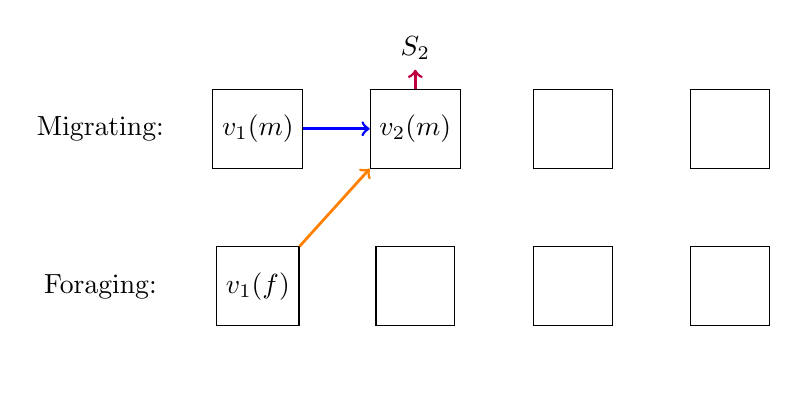
\begin{tikzpicture}[node distance=2cm, block/.style={draw, minimum width=1cm, minimum height=1cm}]

  % First row
  \node[block] (A1) {$v_1(m)$};
  \node[block, right of=A1] (A2) {$v_2(m)$};
  \node[block, right of=A2] (A3) {};
  \node[block, right of=A3] (A4) {};

  % Second row
  \node[block, below of=A1] (B1) {$v_1(f)$};
  \node[block, right of=B1] (B2) {};
  \node[block, right of=B2] (B3) {};
  \node[block, right of=B3] (B4) {};

  % Labels
  \node[coordinate, left of=A1] (J1) {};
  \node[] at (J1) {Migrating:};
  \node[coordinate, left of=B1] (J2) {};
  \node[] at (J2) {Foraging:};

  % Horizontal arrows
  \draw[->, line width=1pt, opacity=1, color=blue] (A1.east) -- (A2.west);
  \draw[->, line width=1pt, opacity=0] (A2.east) -- (A3.west);
  \draw[->, line width=1pt, opacity=0] (A3.east) -- (A4.west);
  \draw[->, line width=1pt, opacity=0] (B1.east) -- (B2.west);
  \draw[->, line width=1pt, opacity=0] (B2.east) -- (B3.west);
  \draw[->, line width=1pt, opacity=0] (B3.east) -- (B4.west);

  % diagonal to blocks
  \draw[->, line width=1pt, opacity=0] (A1.south east) -- (B2.north);
  \draw[->, line width=1pt, opacity=0] (A2.south east) -- (B3.north);
  \draw[->, line width=1pt, opacity=0] (A3.south east) -- (B4.north);
  \draw[->, line width=1pt, opacity=1, color=orange] (B1.north east) -- (A2.south west);
  \draw[->, line width=1pt, opacity=0] (B2.north east) -- (A3.south);
  \draw[->, line width=1pt, opacity=0] (B3.north east) -- (A4.south);

  \node[coordinate, above of=A1, yshift=-1.25cm] (G1) {};
  \node[above] at (G1) {};
  \node[coordinate, above of=A2, yshift=-1.25cm] (G2) {};
  \node[above] at (G2) {$S_2$};
  \node[coordinate, above of=A3, yshift=-1.25cm] (G3) {};
  \node[above] at (G3) {};
  \node[coordinate, above of=A4, yshift=-1.25cm] (G4) {};
  \node[above] at (G4) {};
  \node[coordinate, below of=B1, yshift=1.25cm] (H1) {};
  \node[below] at (H1) {};
  \node[coordinate, below of=B2, yshift=1.25cm] (H2) {};
  \node[below] at (H2) {};
  \node[coordinate, below of=B3, yshift=1.25cm] (H3) {};
  \node[below] at (H3) {};
  \node[coordinate, below of=B4, yshift=1.25cm] (H4) {};
  \node[below] at (H4) {};

  % vertical arrow
  \draw[->, line width=1pt, opacity=1, color=purple] (A2.north) -- (G2.south);

\end{tikzpicture}
\end{center}


\begin{equation*}
\begin{aligned}
    v_2(m) = \max\{&\textcolor{blue}{v_1(m) p(X_2=m | X_1=m)}, \textcolor{orange}{v_1(f) p(X_2=m | X_1=f)} \} \times\\
    &\textcolor{purple}{p(S_2|X_2=m)}.
\end{aligned}
\end{equation*}
    
\end{frame}

\begin{frame}
\frametitle{Viterbi in action}
\begin{center}
\begin{tikzpicture}[node distance=2cm, block/.style={draw, minimum width=1cm, minimum height=1cm}]

  % First row
  \node[block] (A1) {$v_1(m)$};
  \node[block, right of=A1] (A2) {$v_2(m)$};
  \node[block, right of=A2] (A3) {};
  \node[block, right of=A3] (A4) {};

  % Second row
  \node[block, below of=A1] (B1) {$v_1(f)$};
  \node[block, right of=B1] (B2) {};
  \node[block, right of=B2] (B3) {};
  \node[block, right of=B3] (B4) {};

  % Labels
  \node[coordinate, left of=A1] (J1) {};
  \node[] at (J1) {Migrating:};
  \node[coordinate, left of=B1] (J2) {};
  \node[] at (J2) {Foraging:};

  % Horizontal arrows
  \draw[->, line width=1pt, opacity=1, color=blue] (A1.east) -- (A2.west);
  \draw[->, line width=1pt, opacity=0] (A2.east) -- (A3.west);
  \draw[->, line width=1pt, opacity=0] (A3.east) -- (A4.west);
  \draw[->, line width=1pt, opacity=0] (B1.east) -- (B2.west);
  \draw[->, line width=1pt, opacity=0] (B2.east) -- (B3.west);
  \draw[->, line width=1pt, opacity=0] (B3.east) -- (B4.west);

  % Horizontal back-pointers
  \draw[->, line width=1pt, opacity=1, color=cyan, dashed] ($(A2.west)+(0,0.4cm)$) -- ($(A1.east)+(0,0.4cm)$);

  % diagonal to blocks
  \draw[->, line width=1pt, opacity=0] (A1.south east) -- (B2.north);
  \draw[->, line width=1pt, opacity=0] (A2.south east) -- (B3.north);
  \draw[->, line width=1pt, opacity=0] (A3.south east) -- (B4.north);
  \draw[->, line width=1pt, opacity=1, color=orange] (B1.north east) -- (A2.south west);
  \draw[->, line width=1pt, opacity=0] (B2.north east) -- (A3.south);
  \draw[->, line width=1pt, opacity=0] (B3.north east) -- (A4.south);

  \node[coordinate, above of=A1, yshift=-1.25cm] (G1) {};
  \node[above] at (G1) {};
  \node[coordinate, above of=A2, yshift=-1.25cm] (G2) {};
  \node[above] at (G2) {$S_2$};
  \node[coordinate, above of=A3, yshift=-1.25cm] (G3) {};
  \node[above] at (G3) {};
  \node[coordinate, above of=A4, yshift=-1.25cm] (G4) {};
  \node[above] at (G4) {};
  \node[coordinate, below of=B1, yshift=1.25cm] (H1) {};
  \node[below] at (H1) {};
  \node[coordinate, below of=B2, yshift=1.25cm] (H2) {};
  \node[below] at (H2) {};
  \node[coordinate, below of=B3, yshift=1.25cm] (H3) {};
  \node[below] at (H3) {};
  \node[coordinate, below of=B4, yshift=1.25cm] (H4) {};
  \node[below] at (H4) {};

  % vertical arrow
  \draw[->, line width=1pt, opacity=1, color=purple] (A2.north) -- (G2.south);

\end{tikzpicture}
\end{center}


\begin{equation*}
    \text{if } \textcolor{blue}{v_1(m) p(X_2=m | X_1=m)} > \textcolor{orange}{v_1(f) p(X_2=m | X_1=f)}
\end{equation*}
    
\end{frame}

\begin{frame}
\frametitle{Viterbi in action}
\begin{center}
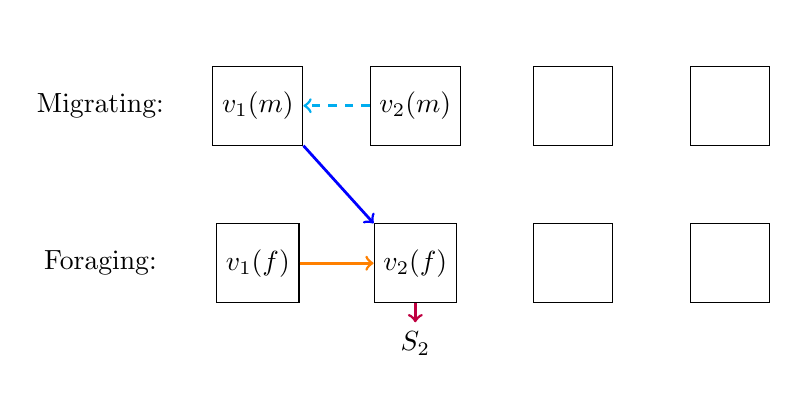
\begin{tikzpicture}[node distance=2cm, block/.style={draw, minimum width=1cm, minimum height=1cm}]

  % First row
  \node[block] (A1) {$v_1(m)$};
  \node[block, right of=A1] (A2) {$v_2(m)$};
  \node[block, right of=A2] (A3) {};
  \node[block, right of=A3] (A4) {};

  % Second row
  \node[block, below of=A1] (B1) {$v_1(f)$};
  \node[block, right of=B1] (B2) {$v_2(f)$};
  \node[block, right of=B2] (B3) {};
  \node[block, right of=B3] (B4) {};

  % Labels
  \node[coordinate, left of=A1] (J1) {};
  \node[] at (J1) {Migrating:};
  \node[coordinate, left of=B1] (J2) {};
  \node[] at (J2) {Foraging:};

  % Horizontal arrows
  \draw[->, line width=1pt, opacity=0, color=blue] (A1.east) -- (A2.west);
  \draw[->, line width=1pt, opacity=1, color=cyan, dashed] (A2.west) -- (A1.east);
  \draw[->, line width=1pt, opacity=0] (A3.east) -- (A4.west);
  \draw[->, line width=1pt, opacity=1, color=orange] (B1.east) -- (B2.west);
  \draw[->, line width=1pt, opacity=0] (B2.east) -- (B3.west);
  \draw[->, line width=1pt, opacity=0] (B3.east) -- (B4.west);

  % diagonal to blocks
  \draw[->, line width=1pt, opacity=1, color=blue] (A1.south east) -- (B2.north west);
  \draw[->, line width=1pt, opacity=0] (A2.south east) -- (B3.north);
  \draw[->, line width=1pt, opacity=0] (A3.south east) -- (B4.north);
  \draw[->, line width=1pt, opacity=0, color=orange] (B1.north east) -- (A2.south west);
  \draw[->, line width=1pt, opacity=0] (B2.north east) -- (A3.south);
  \draw[->, line width=1pt, opacity=0] (B3.north east) -- (A4.south);

  \node[coordinate, above of=A1, yshift=-1.25cm] (G1) {};
  \node[above] at (G1) {};
  \node[coordinate, above of=A2, yshift=-1.25cm] (G2) {};
  \node[above] at (G2) {};
  \node[coordinate, above of=A3, yshift=-1.25cm] (G3) {};
  \node[above] at (G3) {};
  \node[coordinate, above of=A4, yshift=-1.25cm] (G4) {};
  \node[above] at (G4) {};
  \node[coordinate, below of=B1, yshift=1.25cm] (H1) {};
  \node[below] at (H1) {};
  \node[coordinate, below of=B2, yshift=1.25cm] (H2) {};
  \node[below] at (H2) {$S_2$};
  \node[coordinate, below of=B3, yshift=1.25cm] (H3) {};
  \node[below] at (H3) {};
  \node[coordinate, below of=B4, yshift=1.25cm] (H4) {};
  \node[below] at (H4) {};

  % vertical arrow
  \draw[->, line width=1pt, opacity=1, color=purple] (B2.south) -- (H2.north);

\end{tikzpicture}
\end{center}


\begin{equation*}
\begin{aligned}
    v_2(f) = \max\{&\textcolor{blue}{v_1(m) p(X_2=f | X_1=m)}, \textcolor{orange}{v_1(f) p(X_2=f | X_1=f)} \} \times\\
    &\textcolor{purple}{p(S_2|X_2=f)}.
\end{aligned}
\end{equation*}
    
\end{frame}

\begin{frame}
\frametitle{Viterbi in action}
\begin{center}
\begin{tikzpicture}[node distance=2cm, block/.style={draw, minimum width=1cm, minimum height=1cm}]

  % First row
  \node[block] (A1) {$v_1(m)$};
  \node[block, right of=A1] (A2) {$v_2(m)$};
  \node[block, right of=A2] (A3) {};
  \node[block, right of=A3] (A4) {};

  % Second row
  \node[block, below of=A1] (B1) {$v_1(f)$};
  \node[block, right of=B1] (B2) {$v_2(f)$};
  \node[block, right of=B2] (B3) {};
  \node[block, right of=B3] (B4) {};

  % Labels
  \node[coordinate, left of=A1] (J1) {};
  \node[] at (J1) {Migrating:};
  \node[coordinate, left of=B1] (J2) {};
  \node[] at (J2) {Foraging:};

  % Horizontal arrows
  \draw[->, line width=1pt, opacity=0, color=blue] (A1.east) -- (A2.west);
  \draw[->, line width=1pt, opacity=1, color=cyan, dashed] (A2.west) -- (A1.east);
  \draw[->, line width=1pt, opacity=0] (A3.east) -- (A4.west);
  \draw[->, line width=1pt, opacity=1, color=orange] (B1.east) -- (B2.west);
  \draw[->, line width=1pt, opacity=0] (B2.east) -- (B3.west);
  \draw[->, line width=1pt, opacity=0] (B3.east) -- (B4.west);

  % Back-pointers
  \draw[->, line width=1pt, opacity=1, color=cyan, dashed] ($(B2.north west)+(0.2cm,0.2cm)$) -- ($(A1.south east)+(0.2cm,0.2cm)$);
  

  % diagonal to blocks
  \draw[->, line width=1pt, opacity=1, color=blue] (A1.south east) -- (B2.north west);
  \draw[->, line width=1pt, opacity=0] (A2.south east) -- (B3.north);
  \draw[->, line width=1pt, opacity=0] (A3.south east) -- (B4.north);
  \draw[->, line width=1pt, opacity=0, color=orange] (B1.north east) -- (A2.south west);
  \draw[->, line width=1pt, opacity=0] (B2.north east) -- (A3.south);
  \draw[->, line width=1pt, opacity=0] (B3.north east) -- (A4.south);

  \node[coordinate, above of=A1, yshift=-1.25cm] (G1) {};
  \node[above] at (G1) {};
  \node[coordinate, above of=A2, yshift=-1.25cm] (G2) {};
  \node[above] at (G2) {};
  \node[coordinate, above of=A3, yshift=-1.25cm] (G3) {};
  \node[above] at (G3) {};
  \node[coordinate, above of=A4, yshift=-1.25cm] (G4) {};
  \node[above] at (G4) {};
  \node[coordinate, below of=B1, yshift=1.25cm] (H1) {};
  \node[below] at (H1) {};
  \node[coordinate, below of=B2, yshift=1.25cm] (H2) {};
  \node[below] at (H2) {$S_2$};
  \node[coordinate, below of=B3, yshift=1.25cm] (H3) {};
  \node[below] at (H3) {};
  \node[coordinate, below of=B4, yshift=1.25cm] (H4) {};
  \node[below] at (H4) {};

  % vertical arrow
  \draw[->, line width=1pt, opacity=1, color=purple] (B2.south) -- (H2.north);

\end{tikzpicture}
\end{center}


\begin{equation*}
    \text{if } \textcolor{blue}{v_1(m) p(X_2=f | X_1=m)} > \textcolor{orange}{v_1(f) p(X_2=f | X_1=f)}
\end{equation*}
    
\end{frame}

\begin{frame}
\frametitle{Viterbi in action}
\begin{center}
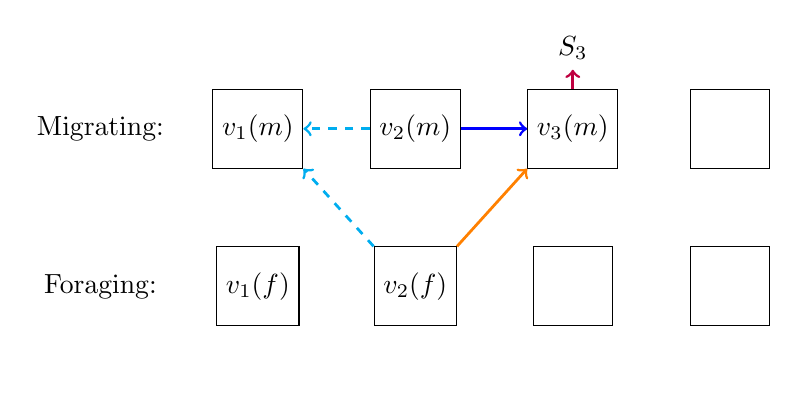
\begin{tikzpicture}[node distance=2cm, block/.style={draw, minimum width=1cm, minimum height=1cm}]

  % First row
  \node[block] (A1) {$v_1(m)$};
  \node[block, right of=A1] (A2) {$v_2(m)$};
  \node[block, right of=A2] (A3) {$v_3(m)$};
  \node[block, right of=A3] (A4) {};

  % Second row
  \node[block, below of=A1] (B1) {$v_1(f)$};
  \node[block, right of=B1] (B2) {$v_2(f)$};
  \node[block, right of=B2] (B3) {};
  \node[block, right of=B3] (B4) {};

  % Labels
  \node[coordinate, left of=A1] (J1) {};
  \node[] at (J1) {Migrating:};
  \node[coordinate, left of=B1] (J2) {};
  \node[] at (J2) {Foraging:};

  % Horizontal arrows
  \draw[->, line width=1pt, opacity=0, color=blue] (A1.east) -- (A2.west);
  \draw[->, line width=1pt, opacity=1, color=cyan, dashed] (A2.west) -- (A1.east);
  \draw[->, line width=1pt, opacity=1, color=blue] (A2.east) -- (A3.west);
  \draw[->, line width=1pt, opacity=0, color=orange] (B1.east) -- (B2.west);
  \draw[->, line width=1pt, opacity=0] (B2.east) -- (B3.west);
  \draw[->, line width=1pt, opacity=0] (B3.east) -- (B4.west);

  % Back-pointers
  

  % diagonal to blocks
  \draw[->, line width=1pt, opacity=1, color=cyan, dashed] (B2.north west) -- (A1.south east);
  \draw[->, line width=1pt, opacity=0] (A2.south east) -- (B3.north);
  \draw[->, line width=1pt, opacity=0] (A3.south east) -- (B4.north);
  \draw[->, line width=1pt, opacity=0, color=orange] (B1.north east) -- (A2.south west);
  \draw[->, line width=1pt, opacity=1, color=orange] (B2.north east) -- (A3.south west);
  \draw[->, line width=1pt, opacity=0] (B3.north east) -- (A4.south);

  \node[coordinate, above of=A1, yshift=-1.25cm] (G1) {};
  \node[above] at (G1) {};
  \node[coordinate, above of=A2, yshift=-1.25cm] (G2) {};
  \node[above] at (G2) {};
  \node[coordinate, above of=A3, yshift=-1.25cm] (G3) {};
  \node[above] at (G3) {$S_3$};
  \node[coordinate, above of=A4, yshift=-1.25cm] (G4) {};
  \node[above] at (G4) {};
  \node[coordinate, below of=B1, yshift=1.25cm] (H1) {};
  \node[below] at (H1) {};
  \node[coordinate, below of=B2, yshift=1.25cm] (H2) {};
  \node[below] at (H2) {};
  \node[coordinate, below of=B3, yshift=1.25cm] (H3) {};
  \node[below] at (H3) {};
  \node[coordinate, below of=B4, yshift=1.25cm] (H4) {};
  \node[below] at (H4) {};

  % vertical arrow
  \draw[->, line width=1pt, opacity=1, color=purple] (A3.north) -- (G3.south);

\end{tikzpicture}
\end{center}


\begin{equation*}
\begin{aligned}
    v_3(m) = \max\{&\textcolor{blue}{v_2(m) p(X_3=m | X_2=m)}, \textcolor{orange}{v_2(f) p(X_3=m | X_2=f)} \} \times\\
    &\textcolor{purple}{p(S_3|X_3=m)}.
\end{aligned}
\end{equation*}
    
\end{frame}

\begin{frame}
\frametitle{Viterbi in action}
\begin{center}
\begin{tikzpicture}[node distance=2cm, block/.style={draw, minimum width=1cm, minimum height=1cm}]

  % First row
  \node[block] (A1) {$v_1(m)$};
  \node[block, right of=A1] (A2) {$v_2(m)$};
  \node[block, right of=A2] (A3) {$v_3(m)$};
  \node[block, right of=A3] (A4) {};

  % Second row
  \node[block, below of=A1] (B1) {$v_1(f)$};
  \node[block, right of=B1] (B2) {$v_2(f)$};
  \node[block, right of=B2] (B3) {};
  \node[block, right of=B3] (B4) {};

  % Labels
  \node[coordinate, left of=A1] (J1) {};
  \node[] at (J1) {Migrating:};
  \node[coordinate, left of=B1] (J2) {};
  \node[] at (J2) {Foraging:};

  % Horizontal arrows
  \draw[->, line width=1pt, opacity=0, color=blue] (A1.east) -- (A2.west);
  \draw[->, line width=1pt, opacity=1, color=cyan, dashed] (A2.west) -- (A1.east);
  \draw[->, line width=1pt, opacity=1, color=blue] (A2.east) -- (A3.west);
  \draw[->, line width=1pt, opacity=0, color=orange] (B1.east) -- (B2.west);
  \draw[->, line width=1pt, opacity=0] (B2.east) -- (B3.west);
  \draw[->, line width=1pt, opacity=0] (B3.east) -- (B4.west);

  % Back-pointers
  \draw[->, line width=1pt, opacity=1, color=cyan, dashed] ($(A3.south west)+(-0.2cm,0cm)$) -- ($(B2.north east)+(-0.2cm,0cm)$);

  % diagonal to blocks
  \draw[->, line width=1pt, opacity=1, color=cyan, dashed] (B2.north west) -- (A1.south east);
  \draw[->, line width=1pt, opacity=0] (A2.south east) -- (B3.north);
  \draw[->, line width=1pt, opacity=0] (A3.south east) -- (B4.north);
  \draw[->, line width=1pt, opacity=0, color=orange] (B1.north east) -- (A2.south west);
  \draw[->, line width=1pt, opacity=1, color=orange] (B2.north east) -- (A3.south west);
  \draw[->, line width=1pt, opacity=0] (B3.north east) -- (A4.south);

  \node[coordinate, above of=A1, yshift=-1.25cm] (G1) {};
  \node[above] at (G1) {};
  \node[coordinate, above of=A2, yshift=-1.25cm] (G2) {};
  \node[above] at (G2) {};
  \node[coordinate, above of=A3, yshift=-1.25cm] (G3) {};
  \node[above] at (G3) {$S_3$};
  \node[coordinate, above of=A4, yshift=-1.25cm] (G4) {};
  \node[above] at (G4) {};
  \node[coordinate, below of=B1, yshift=1.25cm] (H1) {};
  \node[below] at (H1) {};
  \node[coordinate, below of=B2, yshift=1.25cm] (H2) {};
  \node[below] at (H2) {};
  \node[coordinate, below of=B3, yshift=1.25cm] (H3) {};
  \node[below] at (H3) {};
  \node[coordinate, below of=B4, yshift=1.25cm] (H4) {};
  \node[below] at (H4) {};

  % vertical arrow
  \draw[->, line width=1pt, opacity=1, color=purple] (A3.north) -- (G3.south);

\end{tikzpicture}
\end{center}

\begin{equation*}
    \text{if } \textcolor{orange}{v_2(f) p(X_3=m | X_2=f)} > \textcolor{blue}{v_2(m) p(X_3=m | X_2=m)}
\end{equation*}
    
\end{frame}

\begin{frame}
\frametitle{Viterbi in action}
\begin{center}
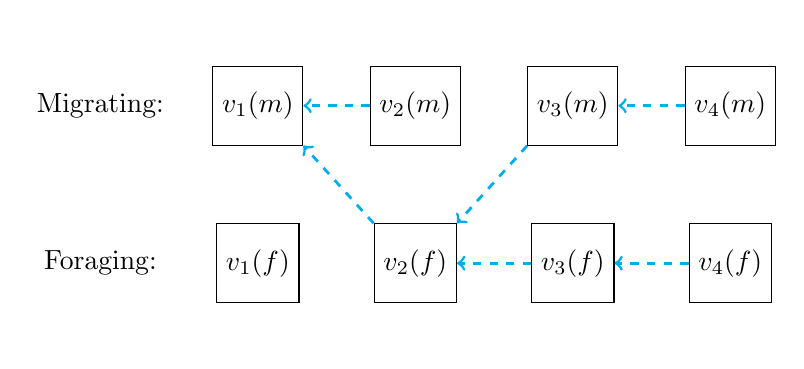
\begin{tikzpicture}[node distance=2cm, block/.style={draw, minimum width=1cm, minimum height=1cm}]

  % First row
  \node[block] (A1) {$v_1(m)$};
  \node[block, right of=A1] (A2) {$v_2(m)$};
  \node[block, right of=A2] (A3) {$v_3(m)$};
  \node[block, right of=A3] (A4) {$v_4(m)$};

  % Second row
  \node[block, below of=A1] (B1) {$v_1(f)$};
  \node[block, right of=B1] (B2) {$v_2(f)$};
  \node[block, right of=B2] (B3) {$v_3(f)$};
  \node[block, right of=B3] (B4) {$v_4(f)$};

  % Labels
  \node[coordinate, left of=A1] (J1) {};
  \node[] at (J1) {Migrating:};
  \node[coordinate, left of=B1] (J2) {};
  \node[] at (J2) {Foraging:};

  % Horizontal arrows
  \draw[->, line width=1pt, opacity=0, color=blue] (A1.east) -- (A2.west);
  \draw[->, line width=1pt, opacity=1, color=cyan, dashed] (A2.west) -- (A1.east);
  \draw[->, line width=1pt, opacity=0, color=blue] (A2.east) -- (A3.west);
  \draw[->, line width=1pt, opacity=1, color=cyan, dashed] (A4.west) -- (A3.east);
  \draw[->, line width=1pt, opacity=0, color=orange] (B1.east) -- (B2.west);
  \draw[->, line width=1pt, opacity=1, color=cyan, dashed] (B3.west) -- (B2.east);
  \draw[->, line width=1pt, opacity=1, color=cyan, dashed] (B4.west) -- (B3.east);

  % diagonal to blocks
  \draw[->, line width=1pt, opacity=1, color=cyan, dashed] (B2.north west) -- (A1.south east);
  \draw[->, line width=1pt, opacity=0] (A2.south east) -- (B3.north);
  \draw[->, line width=1pt, opacity=0] (A3.south east) -- (B4.north);
  \draw[->, line width=1pt, opacity=0, color=orange] (B1.north east) -- (A2.south west);
  \draw[->, line width=1pt, opacity=1, color=cyan, dashed] (A3.south west) -- (B2.north east);
  \draw[->, line width=1pt, opacity=0] (B3.north east) -- (A4.south);

  \node[coordinate, above of=A1, yshift=-1.25cm] (G1) {};
  \node[above] at (G1) {};
  \node[coordinate, above of=A2, yshift=-1.25cm] (G2) {};
  \node[above] at (G2) {};
  \node[coordinate, above of=A3, yshift=-1.25cm] (G3) {};
  \node[above] at (G3) {};
  \node[coordinate, above of=A4, yshift=-1.25cm] (G4) {};
  \node[above] at (G4) {};
  \node[coordinate, below of=B1, yshift=1.25cm] (H1) {};
  \node[below] at (H1) {};
  \node[coordinate, below of=B2, yshift=1.25cm] (H2) {};
  \node[below] at (H2) {};
  \node[coordinate, below of=B3, yshift=1.25cm] (H3) {};
  \node[below] at (H3) {};
  \node[coordinate, below of=B4, yshift=1.25cm] (H4) {};
  \node[below] at (H4) {};


\end{tikzpicture}
\end{center}
    
\end{frame}

\begin{frame}
\frametitle{Viterbi in action}
\begin{center}
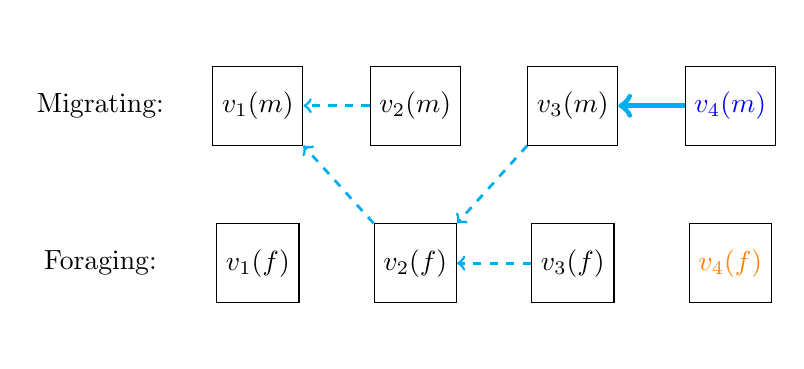
\begin{tikzpicture}[node distance=2cm, block/.style={draw, minimum width=1cm, minimum height=1cm}]

  % First row
  \node[block] (A1) {$v_1(m)$};
  \node[block, right of=A1] (A2) {$v_2(m)$};
  \node[block, right of=A2] (A3) {$v_3(m)$};
  \node[block, right of=A3] (A4) {$\textcolor{blue}{v_4(m)}$};

  % Second row
  \node[block, below of=A1] (B1) {$v_1(f)$};
  \node[block, right of=B1] (B2) {$v_2(f)$};
  \node[block, right of=B2] (B3) {$v_3(f)$};
  \node[block, right of=B3] (B4) {$\textcolor{orange}{v_4(f)}$};

  % Labels
  \node[coordinate, left of=A1] (J1) {};
  \node[] at (J1) {Migrating:};
  \node[coordinate, left of=B1] (J2) {};
  \node[] at (J2) {Foraging:};

  % Horizontal arrows
  \draw[->, line width=1pt, opacity=0, color=blue] (A1.east) -- (A2.west);
  \draw[->, line width=1pt, opacity=1, color=cyan, dashed] (A2.west) -- (A1.east);
  \draw[->, line width=1pt, opacity=0, color=blue] (A2.east) -- (A3.west);
  \draw[->, line width=2pt, opacity=1, color=cyan] (A4.west) -- (A3.east);
  \draw[->, line width=1pt, opacity=0, color=orange] (B1.east) -- (B2.west);
  \draw[->, line width=1pt, opacity=1, color=cyan, dashed] (B3.west) -- (B2.east);
  \draw[->, line width=1pt, opacity=0, color=cyan, dashed] (B4.west) -- (B3.east);

  % diagonal to blocks
  \draw[->, line width=1pt, opacity=1, color=cyan, dashed] (B2.north west) -- (A1.south east);
  \draw[->, line width=1pt, opacity=0] (A2.south east) -- (B3.north);
  \draw[->, line width=1pt, opacity=0] (A3.south east) -- (B4.north);
  \draw[->, line width=1pt, opacity=0, color=orange] (B1.north east) -- (A2.south west);
  \draw[->, line width=1pt, opacity=1, color=cyan, dashed] (A3.south west) -- (B2.north east);
  \draw[->, line width=1pt, opacity=0] (B3.north east) -- (A4.south);

  \node[coordinate, above of=A1, yshift=-1.25cm] (G1) {};
  \node[above] at (G1) {};
  \node[coordinate, above of=A2, yshift=-1.25cm] (G2) {};
  \node[above] at (G2) {};
  \node[coordinate, above of=A3, yshift=-1.25cm] (G3) {};
  \node[above] at (G3) {};
  \node[coordinate, above of=A4, yshift=-1.25cm] (G4) {};
  \node[above] at (G4) {};
  \node[coordinate, below of=B1, yshift=1.25cm] (H1) {};
  \node[below] at (H1) {};
  \node[coordinate, below of=B2, yshift=1.25cm] (H2) {};
  \node[below] at (H2) {};
  \node[coordinate, below of=B3, yshift=1.25cm] (H3) {};
  \node[below] at (H3) {};
  \node[coordinate, below of=B4, yshift=1.25cm] (H4) {};
  \node[below] at (H4) {};


\end{tikzpicture}
\end{center}

\begin{equation*}
    \text{if } \textcolor{blue}{v_4(m)} > \textcolor{orange}{v_4(f)}
\end{equation*}
    
\end{frame}

\begin{frame}
\frametitle{Viterbi in action}
\begin{center}
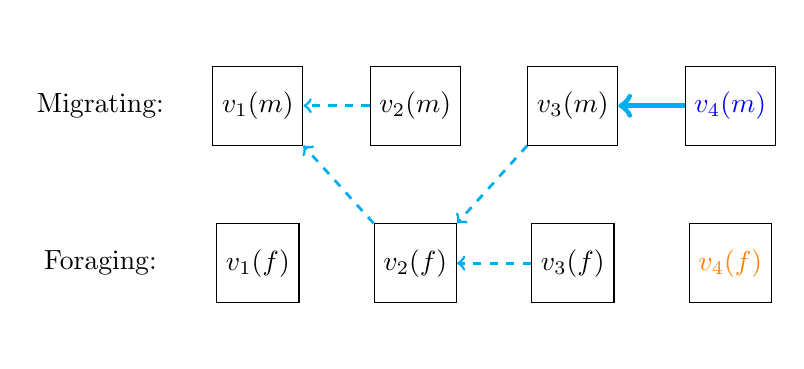
\begin{tikzpicture}[node distance=2cm, block/.style={draw, minimum width=1cm, minimum height=1cm}]

  % First row
  \node[block] (A1) {$v_1(m)$};
  \node[block, right of=A1] (A2) {$v_2(m)$};
  \node[block, right of=A2] (A3) {$v_3(m)$};
  \node[block, right of=A3] (A4) {$\textcolor{blue}{v_4(m)}$};

  % Second row
  \node[block, below of=A1] (B1) {$v_1(f)$};
  \node[block, right of=B1] (B2) {$v_2(f)$};
  \node[block, right of=B2] (B3) {$v_3(f)$};
  \node[block, right of=B3] (B4) {$\textcolor{orange}{v_4(f)}$};

  % Labels
  \node[coordinate, left of=A1] (J1) {};
  \node[] at (J1) {Migrating:};
  \node[coordinate, left of=B1] (J2) {};
  \node[] at (J2) {Foraging:};

  % Horizontal arrows
  \draw[->, line width=1pt, opacity=0, color=blue] (A1.east) -- (A2.west);
  \draw[->, line width=1pt, opacity=1, color=cyan, dashed] (A2.west) -- (A1.east);
  \draw[->, line width=1pt, opacity=0, color=blue] (A2.east) -- (A3.west);
  \draw[->, line width=2pt, opacity=1, color=cyan] (A4.west) -- (A3.east);
  \draw[->, line width=1pt, opacity=0, color=orange] (B1.east) -- (B2.west);
  \draw[->, line width=1pt, opacity=1, color=cyan, dashed] (B3.west) -- (B2.east);
  \draw[->, line width=1pt, opacity=0, color=cyan, dashed] (B4.west) -- (B3.east);

  % diagonal to blocks
  \draw[->, line width=1pt, opacity=1, color=cyan, dashed] (B2.north west) -- (A1.south east);
  \draw[->, line width=1pt, opacity=0] (A2.south east) -- (B3.north);
  \draw[->, line width=1pt, opacity=0] (A3.south east) -- (B4.north);
  \draw[->, line width=1pt, opacity=0, color=orange] (B1.north east) -- (A2.south west);
  \draw[->, line width=1pt, opacity=1, color=cyan, dashed] (A3.south west) -- (B2.north east);
  \draw[->, line width=1pt, opacity=0] (B3.north east) -- (A4.south);

  \node[coordinate, above of=A1, yshift=-1.25cm] (G1) {};
  \node[above] at (G1) {};
  \node[coordinate, above of=A2, yshift=-1.25cm] (G2) {};
  \node[above] at (G2) {};
  \node[coordinate, above of=A3, yshift=-1.25cm] (G3) {};
  \node[above] at (G3) {};
  \node[coordinate, above of=A4, yshift=-1.25cm] (G4) {};
  \node[above] at (G4) {};
  \node[coordinate, below of=B1, yshift=1.25cm] (H1) {};
  \node[below] at (H1) {};
  \node[coordinate, below of=B2, yshift=1.25cm] (H2) {};
  \node[below] at (H2) {};
  \node[coordinate, below of=B3, yshift=1.25cm] (H3) {};
  \node[below] at (H3) {};
  \node[coordinate, below of=B4, yshift=1.25cm] (H4) {};
  \node[below] at (H4) {};


\end{tikzpicture}
\end{center}

\begin{equation*}
    \text{if } \textcolor{blue}{v_4(m)} > \textcolor{orange}{v_4(f)}
\end{equation*}
    
\end{frame}

\begin{frame}
\frametitle{Viterbi in action}
\begin{center}
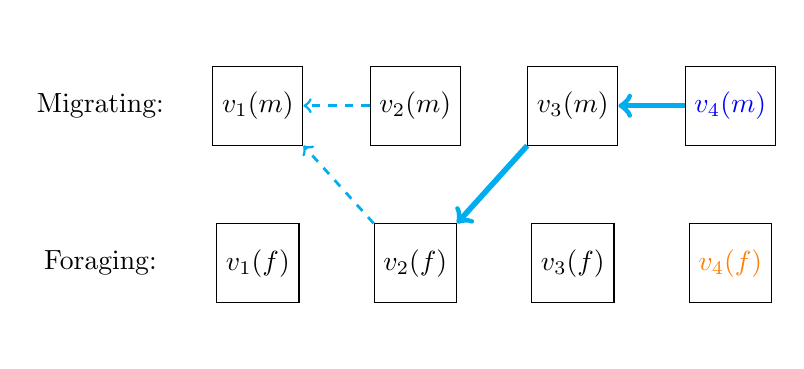
\begin{tikzpicture}[node distance=2cm, block/.style={draw, minimum width=1cm, minimum height=1cm}]

  % First row
  \node[block] (A1) {$v_1(m)$};
  \node[block, right of=A1] (A2) {$v_2(m)$};
  \node[block, right of=A2] (A3) {$v_3(m)$};
  \node[block, right of=A3] (A4) {$\textcolor{blue}{v_4(m)}$};

  % Second row
  \node[block, below of=A1] (B1) {$v_1(f)$};
  \node[block, right of=B1] (B2) {$v_2(f)$};
  \node[block, right of=B2] (B3) {$v_3(f)$};
  \node[block, right of=B3] (B4) {$\textcolor{orange}{v_4(f)}$};

  % Labels
  \node[coordinate, left of=A1] (J1) {};
  \node[] at (J1) {Migrating:};
  \node[coordinate, left of=B1] (J2) {};
  \node[] at (J2) {Foraging:};

  % Horizontal arrows
  \draw[->, line width=1pt, opacity=0, color=blue] (A1.east) -- (A2.west);
  \draw[->, line width=1pt, opacity=1, color=cyan, dashed] (A2.west) -- (A1.east);
  \draw[->, line width=1pt, opacity=0, color=blue] (A2.east) -- (A3.west);
  \draw[->, line width=2pt, opacity=1, color=cyan] (A4.west) -- (A3.east);
  \draw[->, line width=1pt, opacity=0, color=orange] (B1.east) -- (B2.west);
  \draw[->, line width=1pt, opacity=0, color=cyan, dashed] (B3.west) -- (B2.east);
  \draw[->, line width=1pt, opacity=0, color=cyan, dashed] (B4.west) -- (B3.east);

  % diagonal to blocks
  \draw[->, line width=1pt, opacity=1, color=cyan, dashed] (B2.north west) -- (A1.south east);
  \draw[->, line width=1pt, opacity=0] (A2.south east) -- (B3.north);
  \draw[->, line width=1pt, opacity=0] (A3.south east) -- (B4.north);
  \draw[->, line width=1pt, opacity=0, color=orange] (B1.north east) -- (A2.south west);
  \draw[->, line width=2pt, opacity=1, color=cyan] (A3.south west) -- (B2.north east);
  \draw[->, line width=1pt, opacity=0] (B3.north east) -- (A4.south);

  \node[coordinate, above of=A1, yshift=-1.25cm] (G1) {};
  \node[above] at (G1) {};
  \node[coordinate, above of=A2, yshift=-1.25cm] (G2) {};
  \node[above] at (G2) {};
  \node[coordinate, above of=A3, yshift=-1.25cm] (G3) {};
  \node[above] at (G3) {};
  \node[coordinate, above of=A4, yshift=-1.25cm] (G4) {};
  \node[above] at (G4) {};
  \node[coordinate, below of=B1, yshift=1.25cm] (H1) {};
  \node[below] at (H1) {};
  \node[coordinate, below of=B2, yshift=1.25cm] (H2) {};
  \node[below] at (H2) {};
  \node[coordinate, below of=B3, yshift=1.25cm] (H3) {};
  \node[below] at (H3) {};
  \node[coordinate, below of=B4, yshift=1.25cm] (H4) {};
  \node[below] at (H4) {};


\end{tikzpicture}
\end{center}

\begin{equation*}
    \text{if } \textcolor{blue}{v_4(m)} > \textcolor{orange}{v_4(f)}
\end{equation*}
    
\end{frame}

\begin{frame}
\frametitle{Viterbi in action}
\begin{center}
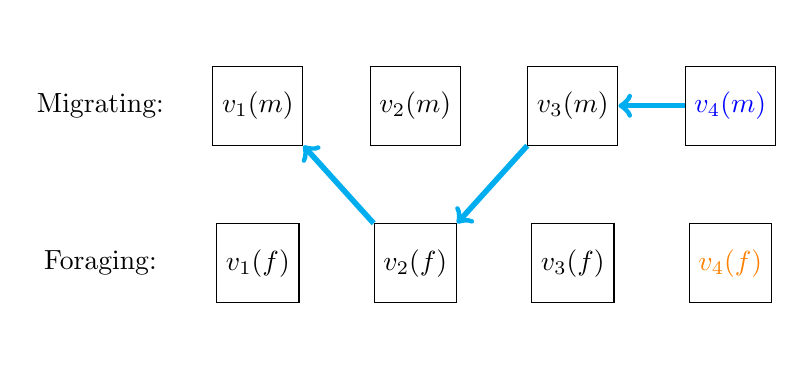
\begin{tikzpicture}[node distance=2cm, block/.style={draw, minimum width=1cm, minimum height=1cm}]

  % First row
  \node[block] (A1) {$v_1(m)$};
  \node[block, right of=A1] (A2) {$v_2(m)$};
  \node[block, right of=A2] (A3) {$v_3(m)$};
  \node[block, right of=A3] (A4) {$\textcolor{blue}{v_4(m)}$};

  % Second row
  \node[block, below of=A1] (B1) {$v_1(f)$};
  \node[block, right of=B1] (B2) {$v_2(f)$};
  \node[block, right of=B2] (B3) {$v_3(f)$};
  \node[block, right of=B3] (B4) {$\textcolor{orange}{v_4(f)}$};

  % Labels
  \node[coordinate, left of=A1] (J1) {};
  \node[] at (J1) {Migrating:};
  \node[coordinate, left of=B1] (J2) {};
  \node[] at (J2) {Foraging:};

  % Horizontal arrows
  \draw[->, line width=1pt, opacity=0, color=blue] (A1.east) -- (A2.west);
  \draw[->, line width=1pt, opacity=0, color=cyan, dashed] (A2.west) -- (A1.east);
  \draw[->, line width=1pt, opacity=0, color=blue] (A2.east) -- (A3.west);
  \draw[->, line width=2pt, opacity=1, color=cyan] (A4.west) -- (A3.east);
  \draw[->, line width=1pt, opacity=0, color=orange] (B1.east) -- (B2.west);
  \draw[->, line width=1pt, opacity=0, color=cyan, dashed] (B3.west) -- (B2.east);
  \draw[->, line width=1pt, opacity=0, color=cyan, dashed] (B4.west) -- (B3.east);

  % diagonal to blocks
  \draw[->, line width=2pt, opacity=1, color=cyan] (B2.north west) -- (A1.south east);
  \draw[->, line width=1pt, opacity=0] (A2.south east) -- (B3.north);
  \draw[->, line width=1pt, opacity=0] (A3.south east) -- (B4.north);
  \draw[->, line width=1pt, opacity=0, color=orange] (B1.north east) -- (A2.south west);
  \draw[->, line width=2pt, opacity=1, color=cyan] (A3.south west) -- (B2.north east);
  \draw[->, line width=1pt, opacity=0] (B3.north east) -- (A4.south);

  \node[coordinate, above of=A1, yshift=-1.25cm] (G1) {};
  \node[above] at (G1) {};
  \node[coordinate, above of=A2, yshift=-1.25cm] (G2) {};
  \node[above] at (G2) {};
  \node[coordinate, above of=A3, yshift=-1.25cm] (G3) {};
  \node[above] at (G3) {};
  \node[coordinate, above of=A4, yshift=-1.25cm] (G4) {};
  \node[above] at (G4) {};
  \node[coordinate, below of=B1, yshift=1.25cm] (H1) {};
  \node[below] at (H1) {};
  \node[coordinate, below of=B2, yshift=1.25cm] (H2) {};
  \node[below] at (H2) {};
  \node[coordinate, below of=B3, yshift=1.25cm] (H3) {};
  \node[below] at (H3) {};
  \node[coordinate, below of=B4, yshift=1.25cm] (H4) {};
  \node[below] at (H4) {};


\end{tikzpicture}
\end{center}

\begin{equation*}
    \text{if } \textcolor{blue}{v_4(m)} > \textcolor{orange}{v_4(f)}
\end{equation*}
    
\end{frame}

\begin{frame}
\frametitle{Viterbi in action}
\begin{center}
\begin{tikzpicture}[node distance=2cm, block/.style={draw, minimum width=1cm, minimum height=1cm}]

  % First row
  \node[block] (A1) {
\includegraphics[width=1cm]{figures/elephant.jpg}};
  \node[block, right of=A1] (A2) {};
  \node[block, right of=A2] (A3) {
\includegraphics[width=1cm]{figures/elephant.jpg}};
  \node[block, right of=A3] (A4) {
\includegraphics[width=1cm]{figures/elephant.jpg}};

  % Second row
  \node[block, below of=A1] (B1) {};
  \node[block, right of=B1] (B2) {
\includegraphics[width=1cm]{figures/elephant.jpg}};
  \node[block, right of=B2] (B3) {};
  \node[block, right of=B3] (B4) {};

  % Labels
  \node[coordinate, left of=A1] (J1) {};
  \node[] at (J1) {Migrating:};
  \node[coordinate, left of=B1] (J2) {};
  \node[] at (J2) {Foraging:};

  % Horizontal arrows
  \draw[->, line width=1pt, opacity=0, color=blue] (A1.east) -- (A2.west);
  \draw[->, line width=1pt, opacity=0, color=cyan, dashed] (A2.west) -- (A1.east);
  \draw[->, line width=1pt, opacity=0, color=blue] (A2.east) -- (A3.west);
  \draw[->, line width=2pt, opacity=1, color=cyan]  (A3.east) -- (A4.west);
  \draw[->, line width=1pt, opacity=0, color=orange] (B1.east) -- (B2.west);
  \draw[->, line width=1pt, opacity=0, color=cyan, dashed] (B3.west) -- (B2.east);
  \draw[->, line width=1pt, opacity=0, color=cyan, dashed] (B4.west) -- (B3.east);

  % diagonal to blocks
  \draw[->, line width=2pt, opacity=1, color=cyan] (A1.south east) -- (B2.north west);
  \draw[->, line width=1pt, opacity=0] (A2.south east) -- (B3.north);
  \draw[->, line width=1pt, opacity=0] (A3.south east) -- (B4.north);
  \draw[->, line width=1pt, opacity=0, color=orange] (B1.north east) -- (A2.south west);
  \draw[->, line width=2pt, opacity=1, color=cyan] (B2.north east) -- (A3.south west);
  \draw[->, line width=1pt, opacity=0] (B3.north east) -- (A4.south);

  \node[coordinate, above of=A1, yshift=-1.25cm] (G1) {};
  \node[above] at (G1) {};
  \node[coordinate, above of=A2, yshift=-1.25cm] (G2) {};
  \node[above] at (G2) {};
  \node[coordinate, above of=A3, yshift=-1.25cm] (G3) {};
  \node[above] at (G3) {};
  \node[coordinate, above of=A4, yshift=-1.25cm] (G4) {};
  \node[above] at (G4) {};
  \node[coordinate, below of=B1, yshift=1.25cm] (H1) {};
  \node[below] at (H1) {};
  \node[coordinate, below of=B2, yshift=1.25cm] (H2) {};
  \node[below] at (H2) {};
  \node[coordinate, below of=B3, yshift=1.25cm] (H3) {};
  \node[below] at (H3) {};
  \node[coordinate, below of=B4, yshift=1.25cm] (H4) {};
  \node[below] at (H4) {};


\end{tikzpicture}
\end{center}

\begin{equation*}
    \text{if } \textcolor{blue}{v_4(m)} > \textcolor{orange}{v_4(f)}
\end{equation*}
    
\end{frame}

\end{document}